\documentclass{article}
\linespread{1.3}
\usepackage[margin=50pt]{geometry}
\usepackage{amsmath, amsthm, amssymb, amsthm, tikz, fancyhdr, graphicx, systeme}
\pagestyle{fancy}
\renewcommand{\headrulewidth}{0pt}
\newcommand{\changefont}{\fontsize{15}{15}\selectfont}

\fancypagestyle{firstpageheader}{
  \fancyhead[R]{
    \changefont
    \parbox[t]{4cm}{ % Adjust width as needed
      Michael Huang\\
      EN.625.633.81\\
      Homework 6
    }
  }
}

\begin{document}

\thispagestyle{firstpageheader}
{\Large 

\section*{1.}

\begin{figure}[h]
    \centering
    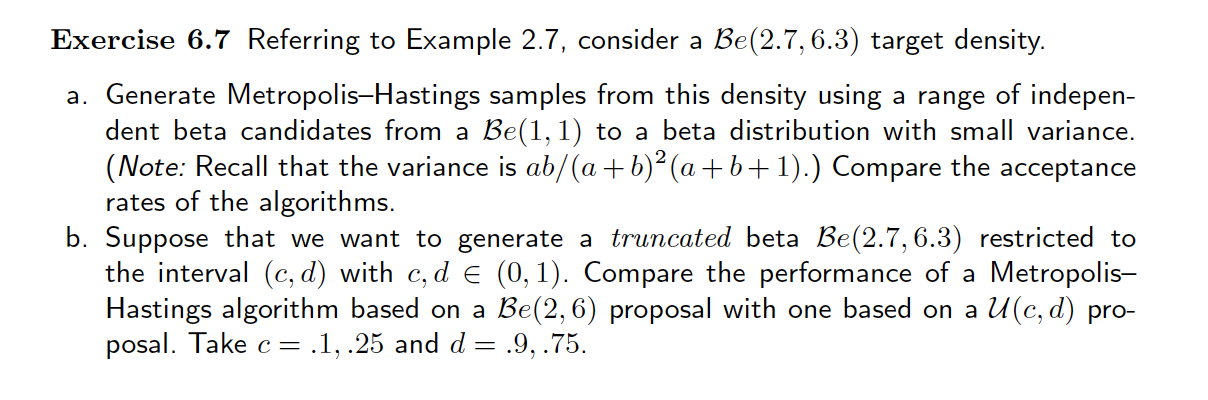
\includegraphics[width=1\textwidth]{Exercise6.7.png}
\end{figure}

\subsection*{(a)} 



\subsection*{(b)}



}
{\Large 

\section*{2.}

\begin{figure}[h]
    \centering
    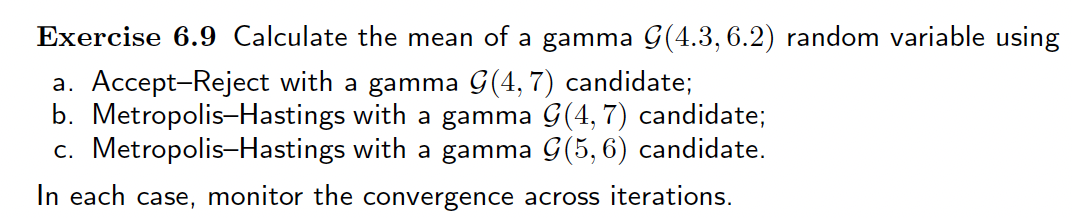
\includegraphics[width=1\textwidth]{Exercise6.9.png}
\end{figure}

\subsection*{(a)} 



\subsection*{(b)}



\subsection*{(c)}



}
{\Large 

\section*{3.}

We show the calculations leading to the kernel expression:
\[
  K(X_t,X_{t+1}) = \rho(X_t,X_{t+1})\,g(X_{t+1}|X_t)  + \delta(X_{t+1}-X_t)\,(1 - r(X_t)).
\]
We know that 
\[
  K(X_t,X_{t+1}) = K(X_t|X_{t+1}) 
\]
To be thorough (and restating the reasoning behind what's given in the notes), we know by definition that the chain either moves to the candidate or doesn't change; i.e. our next state \(X_{t+1}\) is either: \\
- \(X_{cand}\) with probability \(\rho(X_t, X_{cand})\) \\
- \(X_t\) with probability \(1 - \rho(X_t, X_{cand})\) \\
% Given also in the section that \(\delta(z) = 1 \) if \(z = 0\) and 0 otherwise, \\
which translates to the conditional probability density being 
\[
  f(X_{t+1} | X_{cand}, X_t ) = \delta (X_{cand} - X_{t+1}) \rho(X_t, X_{cand}) + \delta(X_t - X_{t+1}) (1 - \rho(X_t, X_{cand}))
\]
as given. We then marginalize over all possible candidate values, i.e. taking
\[
  K(X_t, X_{t+1}) = \int_{\mathbb{R}} f(X_{t+1} | X_{cand} = x_{cand}, X_t) g(X_{cand} = x_{cand}| X_t)dx_{cand}
\]
Plugging in:
\[
  = \int_{\mathbb{R}} [\delta(X_{cand} - X_{t+1}) \rho (X_t, X_{cand}) + \delta(X_t - X_{t+1}) (1 - \rho(X_t, X_{cand})) ] g(x_{cand} | X_t) dx_{cand}
\]
(simplifying a bit, for sanity)
\[
  = \int_{\mathbb{R}} [\delta(x - X_{t+1}) \rho (X_t, x) + \delta(X_t - X_{t+1}) (1 - \rho(X_t, x)) ] g(x | X_t) dx
\]
\[
  = \int_{\mathbb{R}} \delta(x - X_{t+1}) \rho (X_t, x) g(x | X_t) dx + \int_{\mathbb{R}} \delta(X_t - X_{t+1}) (1 - \rho(X_t, x)) g(x | X_t) dx
\]
Looking at the first integral, this essentially represents the sum of all the scenarios where we ended up at \(X_{t+1}\) -- this is due to the product of the delta function representing that we reached the transition or not from the candidate value, the rho function representing the probability of accepting the candidate value, and the g function representing the probability of generating the candidate value. We therefore only care about the actual value of \(x_{cand} = X_{t+1}\), since is the only place under the integral where the delta function is 1 (and nonzero). We can therefore simplify the first term accordingly based on this logic:
\[
  = \rho (X_t, X_{t+1}) g(X_{t+1} | X_t) + \int_{\mathbb{R}} \delta(X_t - X_{t+1}) (1 - \rho(X_t, x)) g(x | X_t) dx
\]
And continuing to integrate:
\[
  = \rho (X_t, X_{t+1}) g(X_{t+1} | X_t) + \delta(X_t - X_{t+1}) \int_{\mathbb{R}} (1 - \rho(X_t, x)) g(x | X_t) dx
\]
\[
  = \rho (X_t, X_{t+1}) g(X_{t+1} | X_t) + \delta(X_t - X_{t+1}) [\int_{\mathbb{R}} g(x | X_t) dx - \int_{\mathbb{R}} \rho(X_t, x) g(x | X_t) dx]
\]
\[
  = \rho (X_t, X_{t+1}) g(X_{t+1} | X_t) + \delta(X_t - X_{t+1}) [1 - \int_{\mathbb{R}} \rho(X_t, x) g(x | X_t) dx]
\]
We now define \(r(X_t) = \int_{\mathbb{R}} \rho(X_t,x)g(x|X_t) dx. \), which represents the combined probability of proposing and accepting some candidate value. We therefore now have 
\[
  = \rho (X_t, X_{t+1}) g(X_{t+1} | X_t) + \delta(X_t - X_{t+1}) (1 - r(X_t))
\]
and because the delta function is symmetric, we have 
\[
  = \rho (X_t, X_{t+1}) g(X_{t+1} | X_t) + \delta(X_{t+1} - X_t) (1 - r(X_t))
\]
exactly as we sought to find.

}
{\Large 

\section*{4.}



}

\end{document}